\chapter{Modified Cut-Tree algorithm by Gusfield}
    Gomory and Hu in their implementation of Cut-Tree use contractions in G to prevent crossings of the cuts. Gusfield provides a simplified version of the same by relaxing the above conditions and arbitrarily separating cuts directly in G without any contractions. Gusfield in his implementation resolves non-crossing cuts using the Non-Crossing Lemma (2). To maintain the reconnection of edges in the \textit{Intermediate Tree} he uses a parent array and another array to represent the weight from a vertex to its parent.

    \section{Intermediate Trees}
    An intermediate tree is a partially formed Gomory-Hu Tree which has not yet completed all the $n-1$ iterations to reach the final state. In an Intermediate Tree represented by $T_* = (V_*,E_*,c_*)$ each node in $V_*$, which consists of original vertices in $V$, by an arbitrary tree of \textit{thin} edges connecting the contained vertices in order to indicate their membership to the node. An edge connecting two nodes in $V_*$ is represented by a \textit{fat} edge in $E_*$, which we connect to an arbitrary vertex in each incident node. Fat edges represent minimum separating cuts in G, and are thus associated with costs. If a node contains only one vertex, we color this vertex black. Black vertices are only incident to at least one thin edge. In this way, $T_* = (V,E_t,E_f,c_f)$ can be also considered as a tree on $V$ with two types of edges (thin edges in $E_t$, fat edges in $E_f$) and vertices (black and white), and a cost function $c_f$ on the fat edges. See figure below:
    
    \begin{figure}[!htb]
        \centering
        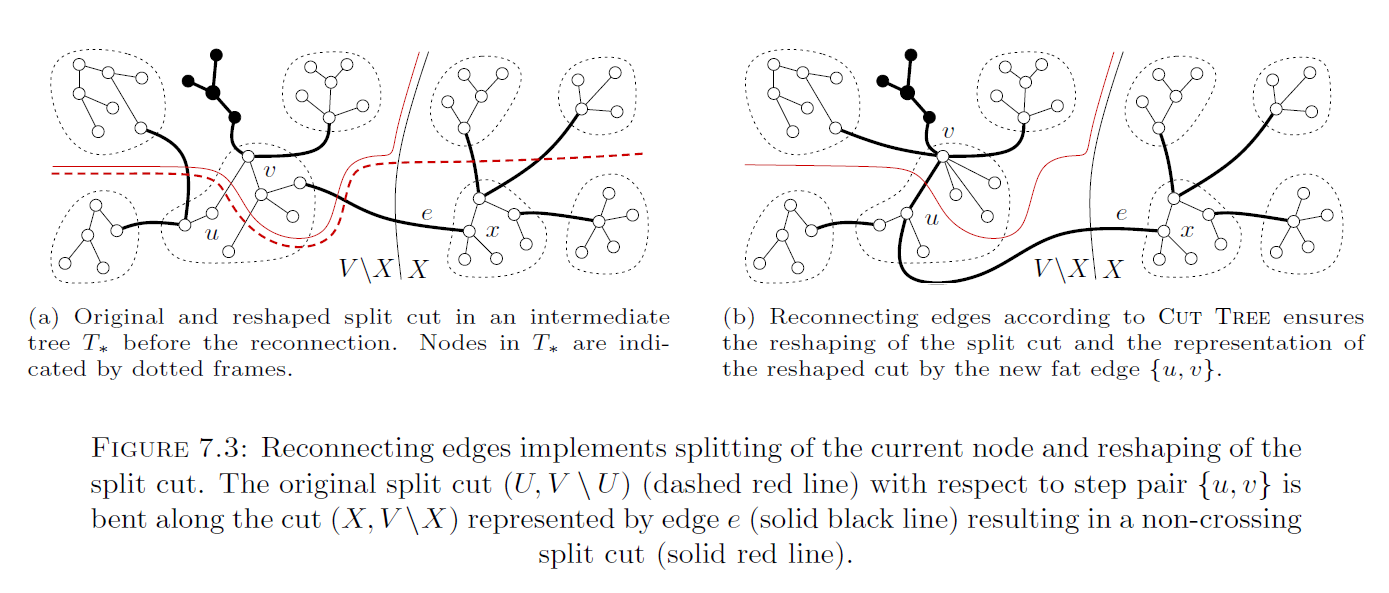
\includegraphics[width=\linewidth]{figures/thin_fat.png}
    \end{figure}

    \section{Description}
    From the above addressing of subtrees of a node using arrays in $T_*$ we can easily address the vertices that are linked by a fat edge to a vertex in the node. As per the representation described above, Algorithm 2 considers the intermediate tree $T_*$ as a tree on the vertices of $G$ consisting of thin and fat edges and bypasses any contraction in $G$. Now, modify Algorithm 1 so that in every intermediate tree, every supernode S contains exactly one node called the \textit{parent/representative} of S, denoted $r(S)$. Then any one node is arbitrarily chosen to be the representative of the first supernode of GH method (Algorithm 1). Next, each successive flow is computed between $r(S)$ and some other vertex $v\in S$. S is split into two supernodes $S_{r(S)}$ and $S_v$. Assign $r(S)$ as the representative of $S_{r(S)}$, and $v$ to be the representative of $S_v$. If $S'$ is a supernode neighbor of $S$ in $T$ before the split, and $r(S')$ falls on the $v$ side of the cut, then replace the $(S,S')$ edge with edge $(S_v,S')$. Now, after $n-1$ iterations each supernode decomposes into a node having only 1 vertex each.

    \vspace{2cm}
    \begin{algorithm}[H]
        \hrulefill
        
        \textbf{Algorithm 2:} Modified Cut-Tree
        
        \hrulefill
        \vspace{2mm}

    \DontPrintSemicolon
    
    \KwIn{Graph $G = (V,E,c)$}
    \KwOut{Cut tree of $G$}
    
    \For{$s \gets 2$ \KwTo $n$}{
        
        Compute a minimum cut between nodes $s$ and $t := p[s]$ in $G$.\;
        Let $X$ be the set of nodes on the $s$-side of the cut.\;
        Output the maximum $s,t$ flow value $f(s,t)$.\;
        
        $fl[s] \gets f(s,t)$\;
    
        \For{$i \gets 1$ \KwTo $n$}{
            \If{$(i \neq s)$ \text{ and } $i \in X$ \text{ and } $p[i] = t$}{
                $p[i] \gets s$\;
            }
        }
    
        \If{$p[t] \in X$}{
            $p[s] \gets p[t]$\;
            $p[t] \gets s$\;
    
            $fl[s] \gets fl[t]$\;
            $fl[t] \gets f(s,t)$\;
        }
    }
    \vspace{2mm}
    \hrulefill
    
    \end{algorithm}


    
    